\documentclass[tikz,border=6pt]{standalone}
\usepackage{amsmath,amssymb}
\usetikzlibrary{calc}
\begin{document}
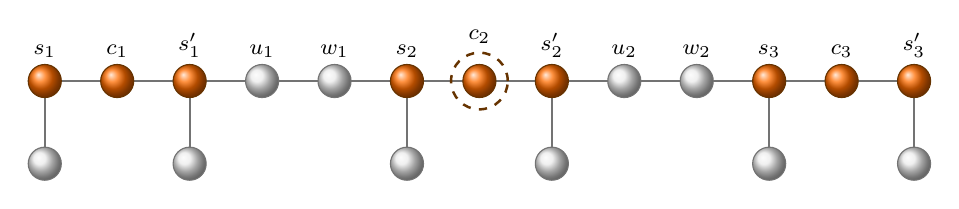
\begin{tikzpicture}[x=0.92cm,y=1cm,
  v/.style={circle,shading=ball,ball color=white!92!black,draw=black!55,minimum size=4.2mm,inner sep=0pt},
  d/.style={v,ball color=orange!85!red,draw=orange!40!black},
  e/.style={draw=black!55,line width=0.8pt},
  lab/.style={font=\footnotesize,inner sep=1pt}]
  % spine s1 c1 s1' u1 w1 s2 c2 s2' u2 w2 s3 c3 s3'
  \foreach \name/\xx in {a1/0,c1/1,b1/2,u1/3,w1/4,a2/5,c2/6,b2/7,u2/8,w2/9,a3/10,c3/11,b3/12}
    \coordinate (\name) at (\xx,0);
  \draw[e] (a1)--(c1)--(b1)--(u1)--(w1)--(a2)--(c2)--(b2)--(u2)--(w2)--(a3)--(c3)--(b3);
  \foreach \j in {1,2,3} {
    \coordinate (la\j) at ($(a\j)+(0,-1.05)$); \coordinate (lb\j) at ($(b\j)+(0,-1.05)$);
    \draw[e] (a\j)--(la\j); \draw[e] (b\j)--(lb\j);
    \node[v] at (la\j) {}; \node[v] at (lb\j) {}; }
  \draw[orange!40!black,line width=0.9pt,dashed] (c2) circle (3.6mm);
  \foreach \p in {u1,w1,u2,w2} \node[v] at (\p) {};
  \foreach \j in {1,2,3} { \node[d] at (a\j) {}; \node[d] at (c\j) {}; \node[d] at (b\j) {}; }
  \foreach \j in {1,2,3} {
    \node[lab,above=2.6mm] at (a\j) {$s_{\j}$};
    \ifnum\j=2 \node[lab,above=4.4mm] at (c\j) {$c_{\j}$}; \else \node[lab,above=2.6mm] at (c\j) {$c_{\j}$}; \fi
    \node[lab,above=2.6mm] at (b\j) {$s'_{\j}$}; }
  \foreach \j in {1,2} { \node[lab,above=2.6mm] at (u\j) {$u_{\j}$}; \node[lab,above=2.6mm] at (w\j) {$w_{\j}$}; }
\end{tikzpicture}
\end{document}
